% Drawing 154/05-2 -- folder 154, batch 05, archive page 84 (PDF page 85).
% Transcription: page de dessin, sans texte : un disque (bord vert clair) traversé d'un arrangement de courbes orange et brunes et de fines lignes grises parallèles (un balayage) ; une bande en zigzag, bordée de brun et coloriée en orange, le traverse de haut en bas, avec une ligne médiane en tirets vert foncé ; deux points opposés du bord sont marqués. C'est une version mise au propre des deux disques du bas de la page 82
% Kind: disk with an arrangement, a sweep and a zigzag band. Method 2 (schematic redraw from the facsimile). Status: partial.
% Notes: A disk (light green rim) crossed by an arrangement of orange and brown curves and by thin parallel grey lines (a sweep); a zigzag band bordered in brown and coloured orange crosses it from top to bottom, with a dark green dashed middle line; two opposite points of the rim are marked. A fair copy of the two lower disks of p. 82. The band's borders and the marked points follow the page view; the orange curves are schematic. Still differs from the facsimile: The band's borders and the marked points follow the page view; the orange curves are schematic.
% Coordinates: 1 unit = 1 mm = 1/100 of the crop width (bbox in page fractions: [0.166, 0.117, 0.479, 0.339]).
% Redrawn by Claude (claude-opus-5-5), issue #73, 2026-11-07; not checked by a human; not compiled (no TeX in the session).
% Revised by Claude (claude-opus-5-5) 2026-11-09 (issue #128) after Michel's check: vertices snapped to exact intersections (drawn points on their lines, meeting ends on the stroke they meet, near-concurrent lines through one computed point, curve ends on their rim); labels at \small as in folder 80 batch 3. Status: partial.
% Rights: reproduces part of the work -- behind RENDER_TRANSCRIPTS, never published by itself.
\documentclass[tikz,border=3pt]{standalone}
\usepackage{amsmath,amssymb}
\usetikzlibrary{patterns,arrows.meta}
\tikzset{Or/.style={orange!90!black}, Ye/.style={yellow!80!orange}, Lg/.style={green!60!black!70}, Dg/.style={green!45!black}, Br/.style={brown!80!black}, Rd/.style={red!85!black}, Bl/.style={blue!70!black}, Gy/.style={black!40}, pencil/.style={black!45}, struck/.style={black!35}, mark/.style={circle,draw,inner sep=1.3pt}, pt/.style={circle,fill,inner sep=0.9pt}, opt/.style={circle,draw,fill=white,inner sep=1.1pt}}
\begin{document}
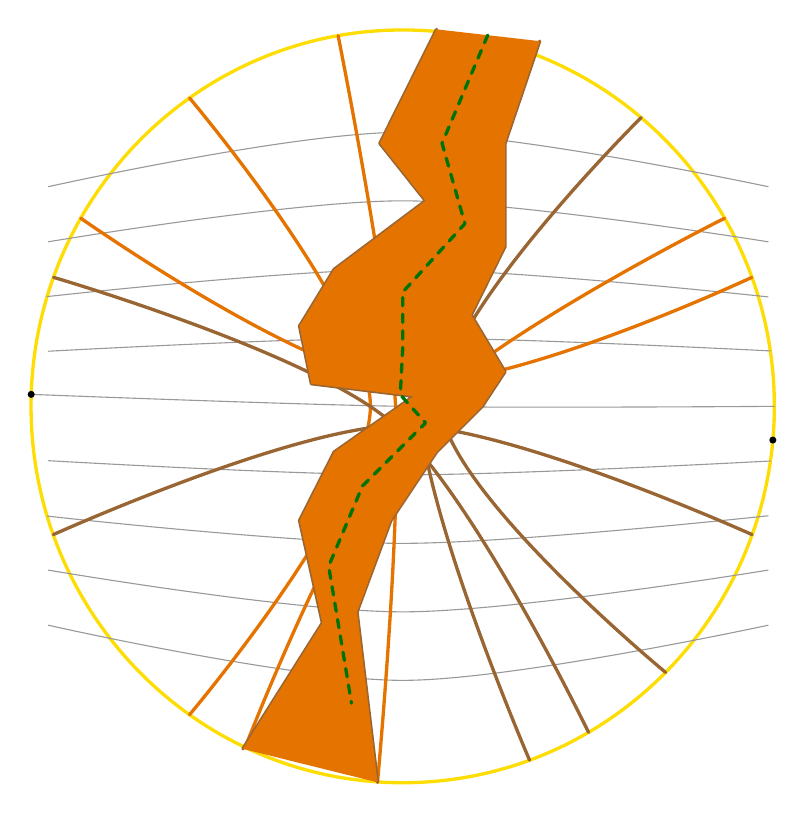
\begin{tikzpicture}[x=1mm,y=1mm,line cap=round,line join=round,font=\scriptsize]
\draw[Ye,very thick] (49.3,-49.3) ellipse[x radius=47.2, y radius=47.8];
\draw[Gy] plot[smooth, tension=0.55] coordinates {(4.3,-21.4) (49.3,-14.5) (95.7,-21.4)};
\draw[Gy] plot[smooth, tension=0.55] coordinates {(4.3,-28.4) (49.3,-23.2) (95.7,-28.4)};
\draw[Gy] plot[smooth, tension=0.55] coordinates {(4.15,-35.36) (49.3,-31.9) (95.7,-35.4)};
\draw[Gy] plot[smooth, tension=0.55] coordinates {(4.3,-42.3) (49.3,-40.6) (95.98,-42.26)};
\draw[Gy] plot[smooth, tension=0.55] coordinates {(2.12,-47.78) (49.3,-49.3) (96.5,-49.3)};
\draw[Gy] plot[smooth, tension=0.55] coordinates {(4.3,-56.2) (49.3,-58) (96,-56.24)};
\draw[Gy] plot[smooth, tension=0.55] coordinates {(4.15,-63.24) (49.3,-66.7) (95.7,-63.2)};
\draw[Gy] plot[smooth, tension=0.55] coordinates {(4.3,-70.1) (49.3,-75.4) (95.7,-70.1)};
\draw[Gy] plot[smooth, tension=0.55] coordinates {(4.3,-77.1) (49.3,-84.1) (95.7,-77.1)};
\draw[Or,very thick] plot[smooth, tension=0.55] coordinates {(41.1,-2.23) (48.4,-49.3) (46.1,-97.05)};
\draw[Br,very thick] plot[smooth, tension=0.55] coordinates {(61.49,-3.12) (51.4,-49.2) (65.41,-94.23)};
\draw[Or,very thick] plot[smooth, tension=0.55] coordinates {(22.23,-10.14) (45.2,-49.3) (22.23,-88.46)};
\draw[Br,very thick] plot[smooth, tension=0.55] coordinates {(79.58,-12.63) (54.1,-49.1) (82.69,-83.09)};
\draw[Or,very thick] plot[smooth, tension=0.55] coordinates {(8.42,-25.41) (49.5,-46.3) (93.64,-32.92)};
\draw[Br,very thick] plot[smooth, tension=0.55] coordinates {(4.93,-65.59) (49.3,-51.7) (93.67,-65.59)};
\draw[Or,very thick] plot[smooth, tension=0.55] coordinates {(90.18,-25.41) (50.8,-50.7) (29.3,-92.6)};
\draw[Br,very thick] plot[smooth, tension=0.55] coordinates {(4.96,-32.92) (47.7,-51.2) (72.9,-90.7)};
\draw[Br,very thick] (53.6,-1.42) -- (46.4,-15.9) -- (52.2,-23.2) -- (40.6,-31.9) -- (36.2,-39.1) -- (37.7,-46.43) -- (50.68,-48.02) -- (40.6,-55.1) -- (36.2,-63.8) -- (39.1,-76.8) -- (29,-92.8);
\draw[Br,very thick] (66.7,-2.92) -- (62.3,-15.9) -- (62.3,-29) -- (58,-37.7) -- (62.3,-44.9) -- (59.4,-49.3) -- (53.6,-55.1) -- (47.8,-63.8) -- (43.5,-75.4) -- (46.1,-97.05);
\fill[pattern=north east lines,Or] (53.6,-1.42) -- (46.4,-15.9) -- (52.2,-23.2) -- (40.6,-31.9) -- (36.2,-39.1) -- (37.7,-46.43) -- (50.68,-48.02) -- (40.6,-55.1) -- (36.2,-63.8) -- (39.1,-76.8) -- (29,-92.8) -- (46.1,-97.05) -- (43.5,-75.4) -- (47.8,-63.8) -- (53.6,-55.1) -- (59.4,-49.3) -- (62.3,-44.9) -- (58,-37.7) -- (62.3,-29) -- (62.3,-15.9) -- (66.7,-2.92) -- cycle;
\draw[Dg,dashed,very thick] (60.1,-2.16) -- (54.3,-15.9) -- (57.2,-26.1) -- (49.3,-34.8) -- (49.3,-42) -- (48.99,-47.81) -- (52.2,-51.4) -- (44.2,-59.4) -- (39.9,-69.6) -- (42.8,-87);
\node[pt] at (2.12,-47.78) {};
\node[pt] at (96.31,-53.58) {};
\end{tikzpicture}
\end{document}
